% Practice Test 09 — Alaska Edition
% Questions: 30 (21 MC + 9 SA)
% Generated by scripts/generate_practice_tests.py

\begin{practiceQuestion}{1-3-q14}{mc}
\begin{questionText}
A recipe uses cups of flour proportional to servings. If $12$ servings need $9$ cups, what is $k$ in cups per serving?
\end{questionText}
\choiceA{$\frac{3}{4}$}
\choiceB{$\frac{4}{3}$}
\choiceC{$3$}
\choiceD{$9$}
\correctAnswer{A}
\explanation{$k = \frac{9}{12} = \frac{3}{4}$ cups per serving.}
\end{practiceQuestion}

\begin{practiceQuestion}{1-5-q10}{mc}
\begin{questionText}
A graph shows that $4$ gallons of paint covers $600$ square feet. The relationship is proportional. How many square feet does $1$ gallon cover?
\end{questionText}
\choiceA{$120$ sq ft}
\choiceB{$150$ sq ft}
\choiceC{$200$ sq ft}
\choiceD{$600$ sq ft}
\correctAnswer{B}
\explanation{Unit rate $= \frac{600}{4} = 150$ sq ft per gallon. This is the $y$-value at $x = 1$ on the graph.}
\end{practiceQuestion}

\begin{practiceQuestion}{1-6-q23}{sa}
\begin{questionText}
A garden hose fills a $60$-gallon tank in $8$ minutes. How long does it take to fill a $225$-gallon tank?
\end{questionText}
\correctAnswer{$30$ minutes}
\explanation{Rate: $60 \div 8 = 7.5$ gal/min. Time: $225 \div 7.5 = 30$ minutes.}
\end{practiceQuestion}

\begin{practiceQuestion}{2-2-q02}{mc}
\begin{questionText}
Use a proportion to find $35\%$ of $120$.
\end{questionText}
\choiceA{$35$}
\choiceB{$38$}
\choiceC{$42$}
\choiceD{$48$}
\correctAnswer{C}
\explanation{Set up $\frac{n}{120} = \frac{35}{100}$. Cross-multiply: $100n = 4200$. Divide: $n = 42$.}
\end{practiceQuestion}

\begin{practiceQuestion}{2-5-q15}{mc}
\begin{questionText}
An art dealer charges $12\%$ commission on each painting sold. If she sold a painting for $\$1{,}500$, what is the revenue for the artist (after the commission is taken)?
\end{questionText}
\choiceA{$\$180$}
\choiceB{$\$1{,}200$}
\choiceC{$\$1{,}320$}
\choiceD{$\$1{,}380$}
\correctAnswer{C}
\explanation{Commission: $1{,}500 \times 0.12 = \$180$. Artist gets: $1{,}500 - 180 = \$1{,}320$.}
\end{practiceQuestion}

\begin{practiceQuestion}{3-1-q06}{mc}
\begin{questionText}
Which list is in order from least to greatest?
\end{questionText}
\choiceA{$-2, \; -5, \; 0, \; 3$}
\choiceB{$-5, \; -2, \; 0, \; 3$}
\choiceC{$3, \; 0, \; -2, \; -5$}
\choiceD{$0, \; -2, \; -5, \; 3$}
\correctAnswer{B}
\explanation{On a number line, numbers increase from left to right: $-5 < -2 < 0 < 3$.}
\end{practiceQuestion}

\begin{practiceQuestion}{3-2-q21}{sa}
\begin{questionText}
A hiker starts at an elevation of $-30$ feet (below sea level). She climbs $45$ feet. What is her new elevation?
\end{questionText}
\correctAnswer{$15$ feet}
\explanation{$(-30) + 45 = 15$. She is now $15$ feet above sea level.}
\end{practiceQuestion}

\begin{practiceQuestion}{3-3-q07}{mc}
\begin{questionText}
What is $(-15) - (-20)$?
\end{questionText}
\choiceA{$-35$}
\choiceB{$35$}
\choiceC{$-5$}
\choiceD{$5$}
\correctAnswer{D}
\explanation{$(-15) - (-20) = (-15) + 20 = 5$.}
\end{practiceQuestion}

\begin{practiceQuestion}{3-10-q19}{sa}
\begin{questionText}
A plane flies at $35{,}000$ feet. It descends $8{,}500$ feet, then climbs $3{,}200$ feet. What is the altitude?
\end{questionText}
\correctAnswer{$29{,}700$ feet}
\explanation{$35{,}000 - 8{,}500 + 3{,}200 = 26{,}500 + 3{,}200 = 29{,}700$ ft.}
\end{practiceQuestion}

\begin{practiceQuestion}{4-1-q28}{gmc}
\begin{questionText}
Look at the input-output table below.

\begin{center}
\begin{tikzpicture}[scale=0.8]
  \node[draw, rounded corners, fill=funOrange!20, minimum width=2.5cm, minimum height=1cm] at (3,0) {\textbf{Rule: ?}};
  \draw[->, thick] (0,0) -- (1.5,0);
  \draw[->, thick] (4.5,0) -- (6,0);
  \node[left] at (0,0) {\textbf{Input}};
  \node[right] at (6,0) {\textbf{Output}};
  % Table
  \node at (0,-1.5) {$1$}; \node at (6,-1.5) {$5$};
  \node at (0,-2.2) {$2$}; \node at (6,-2.2) {$9$};
  \node at (0,-2.9) {$3$}; \node at (6,-2.9) {$13$};
  \node at (0,-3.6) {$4$}; \node at (6,-3.6) {$17$};
\end{tikzpicture}
\end{center}

Which expression represents the rule?
\end{questionText}
\choiceA{$x + 4$}
\choiceB{$5x$}
\choiceC{$4x + 1$}
\choiceD{$3x + 2$}
\correctAnswer{C}
\explanation{Test $x = 1$: $4(1) + 1 = 5$ \checkmark. Test $x = 2$: $4(2) + 1 = 9$ \checkmark. The rule is $4x + 1$.}
\end{practiceQuestion}

\begin{practiceQuestion}{5-2-q26}{gmc}
\begin{questionText}
Look at the balance scale. Both sides are equal. What is the value of $x$?

\begin{center}
\begin{tikzpicture}[scale=0.7]
  % Fulcrum
  \draw[thick] (0,-0.5) -- (-0.4,-1.2) -- (0.4,-1.2) -- cycle;
  % Beam
  \draw[thick] (-4.5,0) -- (4.5,0);
  % Left pan
  \draw[thick] (-4,0) -- (-4.8,-0.6) -- (-3.2,-0.6) -- (-4,0);
  \draw[thick,fill=funBlue!20] (-4.8,-0.6) -- (-4.8,-1) -- (-3.2,-1) -- (-3.2,-0.6) -- cycle;
  % Left contents: 2 boxes and 4 units
  \node[draw,fill=funBlue!40,minimum size=0.4cm] at (-4.4,-1.4) {$x$};
  \node[draw,fill=funBlue!40,minimum size=0.4cm] at (-3.6,-1.4) {$x$};
  \node at (-4,-1.9) {$+ \; 4$};
  % Right pan
  \draw[thick] (4,0) -- (4.8,-0.6) -- (3.2,-0.6) -- (4,0);
  \draw[thick,fill=funOrange!20] (3.2,-0.6) -- (3.2,-1) -- (4.8,-1) -- (4.8,-0.6) -- cycle;
  \node at (4,-1.4) {$18$};
\end{tikzpicture}
\end{center}
\end{questionText}
\choiceA{$x = 9$}
\choiceB{$x = 7$}
\choiceC{$x = 14$}
\choiceD{$x = 11$}
\correctAnswer{B}
\explanation{The equation is $2x + 4 = 18$. Subtract $4$: $2x = 14$. Divide by $2$: $x = 7$.}
\end{practiceQuestion}

\begin{practiceQuestion}{5-3-q03}{mc}
\begin{questionText}
What is the first step to solve $5(x + 2) = 35$ using the ``divide first'' method?
\end{questionText}
\choiceA{Subtract $2$ from both sides}
\choiceB{Distribute $5$ to get $5x + 10 = 35$}
\choiceC{Divide both sides by $5$}
\choiceD{Subtract $5$ from both sides}
\correctAnswer{C}
\explanation{The ``divide first'' method divides both sides by $5$: $x + 2 = 7$.}
\end{practiceQuestion}

\begin{practiceQuestion}{5-4-q10}{mc}
\begin{questionText}
Solve $\dfrac{x}{6} - \dfrac{2}{3} = \dfrac{1}{2}$.
\end{questionText}
\choiceA{$x = 3$}
\choiceB{$x = 7$}
\choiceC{$x = -1$}
\choiceD{$x = 10$}
\correctAnswer{B}
\explanation{Multiply every term by $6$: $x - 4 = 3$. Add $4$: $x = 7$. Check: $\frac{7}{6} - \frac{2}{3} = \frac{7}{6} - \frac{4}{6} = \frac{3}{6} = \frac{1}{2}$ \checkmark.}
\end{practiceQuestion}

\begin{practiceQuestion}{5-5-q28}{gmc}
\begin{questionText}
A store sign shows the rule below. Which inequality represents the sign?

\begin{center}
\begin{tikzpicture}[scale=0.8]
  \draw[thick,rounded corners,fill=funBlue!10] (-0.5,-1.5) rectangle (7,1.5);
  \node[align=center,font=\large] at (3.25,0.4) {\textbf{SALE!}};
  \node[align=center] at (3.25,-0.5) {All items plus $\$5$ tax};
  \node[align=center] at (3.25,-1) {must be \textbf{under} $\$50$};
\end{tikzpicture}
\end{center}

Let $p$ be the price of an item before tax.
\end{questionText}
\choiceA{$p + 5 > 50$}
\choiceB{$p + 5 \leq 50$}
\choiceC{$p + 5 < 50$}
\choiceD{$p + 5 \geq 50$}
\correctAnswer{C}
\explanation{``Under $\$50$'' means strictly less than $50$: $p + 5 < 50$.}
\end{practiceQuestion}

\begin{practiceQuestion}{5-6-q03}{mc}
\begin{questionText}
Solve $x + 5 \geq 9$ and choose the correct graph description.
\end{questionText}
\choiceA{Closed circle at $4$, shade right}
\choiceB{Open circle at $4$, shade right}
\choiceC{Closed circle at $4$, shade left}
\choiceD{Open circle at $14$, shade right}
\correctAnswer{A}
\explanation{Subtract $5$: $x \geq 4$. Closed circle at $4$ (includes $4$), shade right.}
\end{practiceQuestion}

\begin{practiceQuestion}{6-2-q05}{mc}
\begin{questionText}
When you redraw a scale drawing at a smaller scale (more real units per cm), the new drawing is:
\end{questionText}
\choiceA{Larger than the original drawing}
\choiceB{Smaller than the original drawing}
\choiceC{The same size as the original drawing}
\choiceD{A different shape than the original drawing}
\correctAnswer{B}
\explanation{A smaller scale means each cm represents more real distance, so fewer cm are needed. The drawing gets smaller. The shape stays the same.}
\end{practiceQuestion}

\begin{practiceQuestion}{6-3-q02}{mc}
\begin{questionText}
Can you draw a triangle with sides $5$ cm, $5$ cm, and $5$ cm?
\end{questionText}
\choiceA{No, it is impossible}
\choiceB{Yes, exactly one triangle}
\choiceC{Yes, more than one triangle}
\choiceD{Yes, but only if one angle is $90°$}
\correctAnswer{B}
\explanation{All three inequality checks pass ($5 + 5 = 10 > 5$). Three equal sides (SSS) produce exactly one equilateral triangle.}
\end{practiceQuestion}

\begin{practiceQuestion}{6-4-q22}{sa}
\begin{questionText}
A triangle has sides $11$, $13$, and $20$. Does it satisfy the triangle inequality?
\end{questionText}
\correctAnswer{Yes}
\explanation{$11 + 13 = 24 > 20$ \checkmark, $11 + 20 = 31 > 13$ \checkmark, $13 + 20 = 33 > 11$ \checkmark. All three checks pass.}
\end{practiceQuestion}

\begin{practiceQuestion}{6-5-q29}{gsa}
\begin{questionText}
The diagram shows a cylinder with radius $4$ cm and height $9$ cm. A vertical cut is made through the center. Describe the cross-section and give its dimensions.

\begin{center}
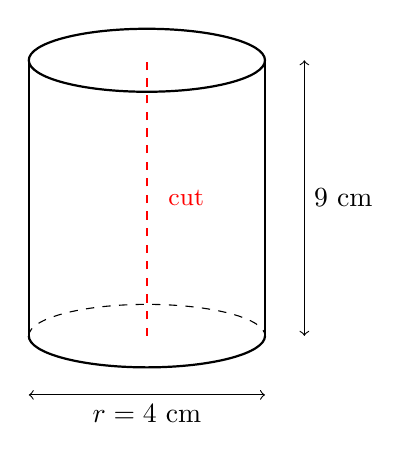
\begin{tikzpicture}[scale=0.5]
  % Cylinder
  \draw[thick] (-3,0) -- (-3,7);
  \draw[thick] (3,0) -- (3,7);
  \draw[thick] (-3,0) arc[start angle=180,end angle=360,x radius=3,y radius=0.8];
  \draw[dashed] (-3,0) arc[start angle=180,end angle=0,x radius=3,y radius=0.8];
  \draw[thick] (-3,7) arc[start angle=180,end angle=360,x radius=3,y radius=0.8];
  \draw[thick] (-3,7) arc[start angle=180,end angle=0,x radius=3,y radius=0.8];
  % Vertical cut line
  \draw[thick,red,dashed] (0,0) -- (0,7);
  \node[right,red] at (0.3,3.5) {\small cut};
  % Labels
  \draw[<->] (-3,-1.5) -- (3,-1.5);
  \node[below] at (0,-1.5) {$r = 4$ cm};
  \draw[<->] (4,0) -- (4,7);
  \node[right] at (4,3.5) {$9$ cm};
\end{tikzpicture}
\end{center}
\end{questionText}
\correctAnswer{Rectangle; $8$ cm by $9$ cm}
\explanation{A vertical cut through the center of a cylinder produces a rectangle. Width = diameter = $2 \times 4 = 8$ cm. Height = $9$ cm.}
\end{practiceQuestion}

\begin{practiceQuestion}{7-3-q12}{mc}
\begin{questionText}
Which circle has the larger area: Circle A with radius $4$ cm or Circle B with diameter $10$ cm?
\end{questionText}
\choiceA{Circle A}
\choiceB{Circle B}
\choiceC{They have the same area}
\choiceD{Not enough information}
\correctAnswer{B}
\explanation{Circle A: $r = 4$, $A = \pi(16) = 50.24$ cm$^2$. Circle B: $r = 5$, $A = \pi(25) = 78.5$ cm$^2$. Circle B is larger.}
\end{practiceQuestion}

\begin{practiceQuestion}{7-4-q03}{mc}
\begin{questionText}
A shape is made of two rectangles. Rectangle A is $6$ m by $3$ m and Rectangle B is $4$ m by $3$ m. What is the total area?
\end{questionText}
\choiceA{$18$ m$^2$}
\choiceB{$24$ m$^2$}
\choiceC{$30$ m$^2$}
\choiceD{$72$ m$^2$}
\correctAnswer{C}
\explanation{Rectangle A: $6 \times 3 = 18$ m$^2$. Rectangle B: $4 \times 3 = 12$ m$^2$. Total: $18 + 12 = 30$ m$^2$.}
\end{practiceQuestion}

\begin{practiceQuestion}{7-5-q23}{sa}
\begin{questionText}
A shipping box is $12$ in by $8$ in by $6$ in. What is the total surface area?
\end{questionText}
\correctAnswer{$432$ in$^2$}
\explanation{$SA = 2(12 \times 8) + 2(12 \times 6) + 2(8 \times 6) = 192 + 144 + 96 = 432$ in$^2$.}
\end{practiceQuestion}

\begin{practiceQuestion}{7-6-q24}{sa}
\begin{questionText}
A planter box is $3$ ft long, $1.5$ ft wide, and $2$ ft deep. How many cubic feet of soil are needed to fill it?
\end{questionText}
\correctAnswer{$9$ ft$^3$}
\explanation{$V = 3 \times 1.5 \times 2 = 9$ ft$^3$.}
\end{practiceQuestion}

\begin{practiceQuestion}{8-1-q19}{sa}
\begin{questionText}
A random sample of $80$ out of $2{,}000$ students found that $20$ students ride the bus. Predict how many students in the school ride the bus.
\end{questionText}
\correctAnswer{$500$}
\explanation{$\frac{20}{80} = 25\%$. Then $25\%$ of $2{,}000 = 500$.}
\end{practiceQuestion}

\begin{practiceQuestion}{8-3-q04}{mc}
\begin{questionText}
Group X has a median of $50$ and a range of $10$. Group Y has a median of $50$ and a range of $30$. Which statement is true?
\end{questionText}
\choiceA{Group X has more data values}
\choiceB{Group Y has a higher center}
\choiceC{Group Y is more spread out than Group X}
\choiceD{The groups are identical}
\correctAnswer{C}
\explanation{Both have the same median, but Group Y's larger range means its data is more spread out.}
\end{practiceQuestion}

\begin{practiceQuestion}{8-4-q01}{mc}
\begin{questionText}
Data set A: $10, 12, 14, 16, 18$. What is the mean?
\end{questionText}
\choiceA{$12$}
\choiceB{$14$}
\choiceC{$16$}
\choiceD{$70$}
\correctAnswer{B}
\explanation{$\frac{10+12+14+16+18}{5} = \frac{70}{5} = 14$.}
\end{practiceQuestion}

\begin{practiceQuestion}{8-7-q07}{mc}
\begin{questionText}
In a double bar graph, Team X scored $30$, $45$, $50$ over three games and Team Y scored $35$, $40$, $55$. What was Team Y's total?
\end{questionText}
\choiceA{$120$}
\choiceB{$125$}
\choiceC{$130$}
\choiceD{$135$}
\correctAnswer{C}
\explanation{$35 + 40 + 55 = 130$.}
\end{practiceQuestion}

\begin{practiceQuestion}{9-4-q25}{sa}
\begin{questionText}
A probability model assigns $P(A) = 0.35$, $P(B) = 0.25$, $P(C) = 0.25$, and $P(D) = 0.20$. Is this a valid model? Explain.
\end{questionText}
\correctAnswer{No}
\explanation{$0.35 + 0.25 + 0.25 + 0.20 = 1.05$, which is greater than $1$. A valid model must have probabilities that sum to exactly $1$.}
\end{practiceQuestion}

\begin{practiceQuestion}{9-6-q14}{mc}
\begin{questionText}
A bag has $4$ green and $6$ yellow marbles. You pick one marble without replacement and then pick another. What is the probability that the first is green and the second is yellow?
\end{questionText}
\choiceA{$\frac{24}{100}$}
\choiceB{$\frac{24}{90}$}
\choiceC{$\frac{4}{15}$}
\choiceD{$\frac{6}{10}$}
\correctAnswer{C}
\explanation{$P(\text{green first}) = \frac{4}{10}$. After removing a green, $P(\text{yellow second}) = \frac{6}{9}$. $P = \frac{4}{10} \times \frac{6}{9} = \frac{24}{90} = \frac{4}{15}$.}
\end{practiceQuestion}

\begin{practiceQuestion}{9-7-q06}{mc}
\begin{questionText}
Why are simulations useful?
\end{questionText}
\choiceA{They always give exact answers}
\choiceB{They can estimate probabilities when real experiments are too difficult or impractical}
\choiceC{They replace all mathematical calculations}
\choiceD{They only work for coin flips}
\correctAnswer{B}
\explanation{Simulations estimate probabilities for complex events that are hard to compute directly or where real experiments are impractical.}
\end{practiceQuestion}
